% Some commands used in this file
\chapter{Preliminaries}
\section{MEMS Microphones}
\acrfull{mems} microphones represent a significant evolution in acoustic technology.
Unlike traditional microphones that rely on larger, more mechanically complex systems,
\acrshort{mems} microphones integrate acoustic sensing elements with electronic circuits on a tiny silicon chip.
These microphones have gained immense popularity due to their compact size, robustness, and cost-effectiveness.
\acrshort{mems} technology allows for the production of microphones with high sound quality and excellent reliability,
making them ideal for a wide range of applications including mobile devices, wearable technology, and \acrshort{iot} devices.
Their small footprint also enables design flexibility in increasingly miniaturized electronic devices.
\acrshort{mems} microphones differ in their output signal types, leading to three categories: analog microphones, \acrshort{pdm} microphones, and \acrshort{pcm} microphones.
\begin{figure}[h]
	\centering
	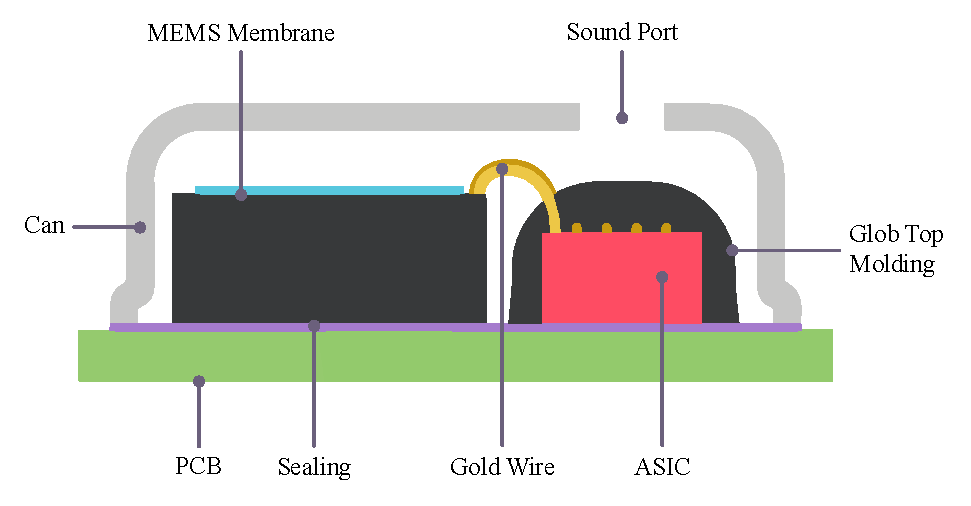
\includegraphics[width=0.9\textwidth]{images/2_preliminaries/mems_microphone_illustration.pdf}
	\caption{Internal structure of a MEMS microphone}
	\label{fig:mems_microphone}
\end{figure}

\subsection{Analog Microphones}
Analog \acrshort{mems} microphones convert sound into an analog electrical signal.
They are simple and easy to integrate in analog circuits but may require additional signal amplification components.
A disadvantage of analog microphones is that they are susceptible to noise and interference, making them unsuitable for long-distance transmission.
\begin{figure}[h!]
	\centering
	\vspace{-0.1cm}
	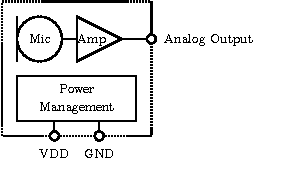
\includegraphics[height=2.9cm, trim={0 0.4cm 0 0}]{images/2_preliminaries/mems_microphone_types_analog.pdf}
	\caption{Block diagram of analog MEMS microphone}
	\label{fig:mems_microphone_types_analog}
\end{figure}

\subsection{PDM Microphones}
\acrshort{pdm} microphones output a digital signal representing the acoustic waveform.
Their digital format is noise-resistant and supports long-distance transmission, making them ideal for multiplexed, multi-microphone setups.
These microphone types require a high-frequency clock signal to operate (typically 1.5\,MHz to 3.25\,MHz),
which must be provided by the host (e.g. a \acrshort{mcu} or \acrshort{fpga}).
A dedicated channel select pin is used to select the microphone's output channel in multiplexed systems.
\begin{figure}[h!]
	\centering
	\vspace{-0.1cm}
	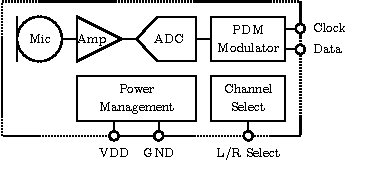
\includegraphics[height=2.9cm, trim={0 0.4cm 0 0}]{images/2_preliminaries/mems_microphone_types_pdm.pdf}
	\caption{Block diagram of PDM MEMS microphone}
	\label{fig:mems_microphone_types_pdm}
\end{figure}

\subsection{PCM Microphones}
\acrshort{pcm} microphones provide a digital output using the \acrlong{pcm} format, most often interfaced via the \acrshort{i2s} protocol.
Compared to \acrshort{pdm} microphones, \acrshort{pcm} microphones have a build-in decimation filter, which simplifies the signal processing chain, as the host no longer needs to perform this task.
However, \acrshort{pcm} microphones are more complex, costly and less common in the industry than \acrshort{pdm} microphones.
\begin{figure}[h!]
	\centering
	\vspace{-0.1cm}
	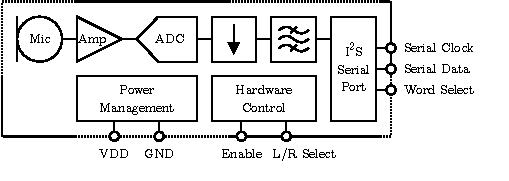
\includegraphics[height=2.9cm, trim={0 0.4cm 0 0}]{images/2_preliminaries/mems_microphone_types_pcm.pdf}
	\caption{Block diagram of PCM MEMS microphone}
	\label{fig:mems_microphone_types_pcm}
\end{figure}
\clearpage

\subsection{Microphone Port Location}
\acrshort{mems} microphones can be categorized based on their port location: top-port and bottom-port.
Top-port microphones have the sound inlet on the top of the package, suitable when the sound source is above the microphone.
Conversely, bottom-port microphones have the inlet at the bottom, ideal for mounting on surfaces where sound comes from the side or below.
For bottom-port microphones, the sound must travel through a hole in the \acrshort{pcb} to reach the microphone, which can affect the sound quality.
\begin{figure}[h!]
	\centering
	\begin{minipage}{0.49\textwidth}
		\centering
		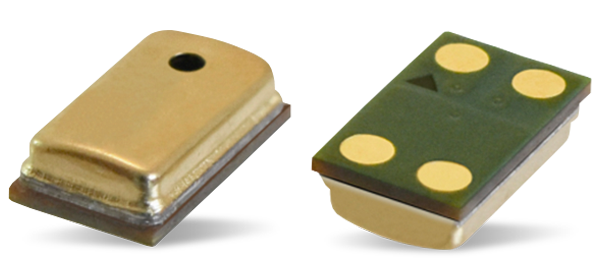
\includegraphics[width=\textwidth]{images/2_preliminaries/mems_microphone_top.png}
		\caption{Top-port MEMS microphone}
		\label{fig:mems_microphone_top}
	\end{minipage}
	\begin{minipage}{0.49\textwidth}
		\centering
		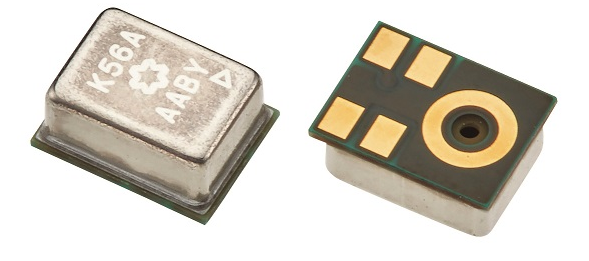
\includegraphics[width=\textwidth]{images/2_preliminaries/mems_microphone_bottom.png}
		\caption{Bottom-port MEMS microphone}
		\label{fig:mems_microphone_bottom}
	\end{minipage}
\end{figure}


\section{Pulse Density Modulation (PDM)}
\acrfull{pdm} is a form of modulation used to represent an analog signal with a binary sequence.
In \acrshort{mems} microphones, \acrshort{pdm} is particularly popular due to its simplicity and efficiency.
The microphone's diaphragm movements modulate a high-frequency carrier signal,
resulting in a digital output with a density of pulses corresponding to the amplitude of the input signal.
The main advantage of PDM in \acrshort{mems} microphones is its resilience to noise and interference,
making it ideal for long cable runs and complex electronic environments.
Additionally, \acrshort{pdm} simplifies the microphone's design, allowing for smaller and more power-efficient microphones.
However, it requires a decimation filter in the signal processing chain to convert the high-frequency pulse sequence into a usable digital audio signal.

\section{Time Division Multiplexing (TDM)}
\acrfull{tdm} is a method of transmitting and receiving independent signals over a common signal path by means of synchronized switches at each end of the transmission line.
In the context of digital audio, \acrshort{tdm} allows multiple audio streams to share a single communication line,
with each stream getting a dedicated time slot. This technique is valuable in systems where multiple audio channels,
such as in surround sound systems or multi-microphone arrays, need to be transmitted over a single cable.
\acrshort{tdm}'s main advantage is its ability to efficiently handle multiple audio streams without the need for multiple physical connections.
This makes it particularly useful in professional audio applications, broadcast systems, and complex audio setups.
However, \acrshort{tdm} systems can be more complex to implement and require precise synchronization to ensure that the timing of the different channels is maintained.
